\chapter{L'amplificateur opérationnel}
\setcounter{section}{-1}
\section{Pourquoi amplifier}
L'amplification est omniprésente en électronique analogique. On la réalise avec l'\textit{amplificateur-opérationnel} (composant) bien que le \textit{transistor} soit également fondamentalement un amplificateur. Trois des $6*10^{34}$ raisons d'amplifier sont par exemple : 
\begin{enumerate}
	\item Signaux très faibles
	\item Réglage de niveau
	\item Amplification en amont d'un convertisseur analogique/numérique (CAN)
\end{enumerate}

Dans une table de mixage analogique, le signal initial étant relativement faible (venant par exemple d'un micro), les \textit{pré-amplis} servent à augmenter son niveau vis-à-vis des parasites. Ensuite, dans chaque voie, des \textit{amplis} servent à régler le niveau des signaux (pour le mixage).



\section{Ampli-op : propriétés de base}
\subsection{Qu'est ce qu'un ampli-op ?}
\begin{wrapfigure}[5]{r}{2cm}
	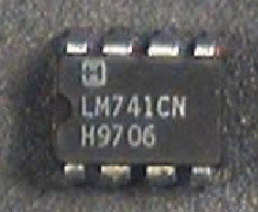
\includegraphics[scale=0.25]{img/image37}
	\captionof{figure}{AOP}
\end{wrapfigure}

Un ampli-op se présente le plus classiquement sous forme d'un circuit intégré à huit "pattes". Il s'agit d'un composant à \textbf{deux} bornes d'entrée et \textbf{une} borne de sortie. Conventionnellement, en électronique analogique, le triangle est son symbole.
\begin{center}
	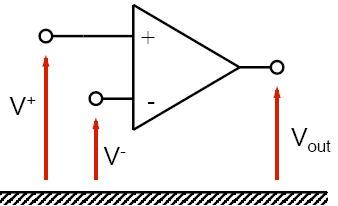
\includegraphics[scale=0.4]{img/image38}
	\captionof{figure}{Représentation schématique d'un AOP}
\end{center}
Les deux bornes sont respectivement notée "+" et "-" et correspondent respectivement à l'\textit{entrée non-inverseuse} et à l'\textit{entrée inverseuse}.

\subsubsection{Tension d'entrée et de sortie}
Chacune des \textit{entrées} reçoit un signal de tension mesurée par rapport à la masse : $V^+$ et $V^-$. Même topo pour la tension de sortie $V_{out}$.\\
La fonction d'un AOP est d'amplifier la \textbf{différence} $V_d$ des tensions présentes à ses bornes. Il s'agit de la \textit{tension d'entrée différentielle.\footnote{On retrouve la notion de tension différentielle vue au cours \textit{Électricité : ELEC-H200} signifiant ici qu'aucune des deux bornes n'est la masse.}}

\subsubsection{Loi fondamentale et gain}
Cette fonction d'amplification se traduit mathématiquement par la loi : 
\begin{equation}
	V_{out} = A.V_d
\end{equation}
où $A$ est le gain de l'AOP, c'est à dire le facteur\footnote{Sans dimension.} d'amplification de son entrée différentielle et sa sortie.\\
Quelques remarque importantes sont à considérer :
\begin{itemize}
	\item Le gain $A$ est toujours très élevé : 30,000 à 100,000 $\rightarrow$ il sera considéré infini.
	\item Un tel gain n'a de sens que si le signal d'entrée est très faible : c'est le cas pour $V_d$ ($\ll 1\ mV$).
	\item $V_d$ et $V_{out}$ sont de signes quelconques.
\end{itemize}
Le schéma ci-dessous récapitule les concepts précédents et les deux relations à retenir :
\begin{center}
	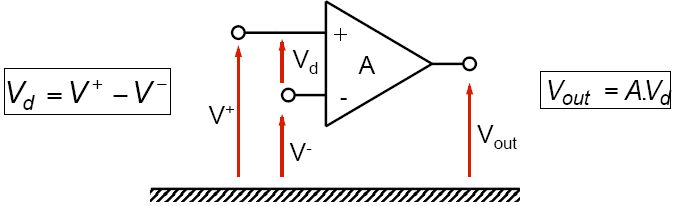
\includegraphics[scale=0.5]{img/image39}
	\captionof{figure}{Schéma de synthèse}
\end{center}


\subsubsection{Tensions et bornes d'alimentation}
\begin{wrapfigure}[8]{l}{3cm}
	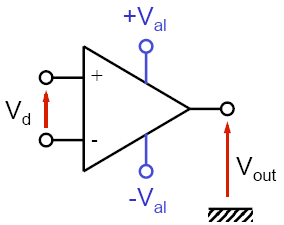
\includegraphics[scale=0.3]{img/image40}
	\captionof{figure}{Alimentation}
\end{wrapfigure}
Afin d'amplifier le signal, l'AOP doit être lui même alimenté en énergie : il possède en plus de ses bornes d'entrée et de sortie des bornes d'alimentations $+V_{al}$ et $-V_{al}$. \\

Ces tensions à fournir sont le plus souvent symétriques et valent typiquement +12V/-12V ou +15V/-15V. L'AOP est donc un composé \textit{actif}.\\

Un \textit{quadripôle actif} est défini par le fait qu'un signal de puissance élevée (sortie) est contrôlé par un signal de puissance plus faible (entrée), ce qui est typiquement le cas de notre AOP.\\

\prop{La tension de sortie ne peut pas sortir de la gamme fixée par ces tensions d'alimentations.
	\begin{equation}
		-V_{al} \leq V_{out} \leq V_{al}
	\end{equation}}



\newpage

\subsection{Impédances d'entrée et de sortie}\begin{wrapfigure}[1]{r}{3cm}
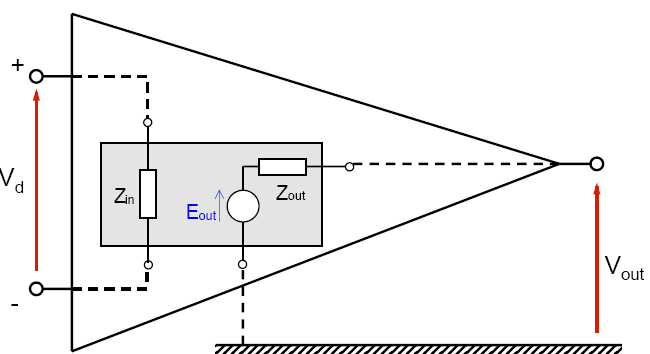
\includegraphics[scale=0.23]{img/image41}
\captionof{figure}{E. Thévenin}
\end{wrapfigure}
\subsubsection{Équivalent de Thévenin}

Pour modéliser l'équivalent de Thévenin, il faut tenir compte de deux particularités de l'AOP :
\begin{enumerate}
	\item L'impédance d'entrée $Z_{in}$ est différentielle
	\item Au contraire, la source $E_{out}$ est référencée à la masse.
\end{enumerate}


\subsubsection{Valeur des impédances}
L'impédance d'entrée (différentielle) d'un AOP est \textbf{très élevée} ($>\ 10\ M\Omega$). Cela à pour conséquence que le courant circulant entre la borne "+" et "-" est très faible. On considèrera cette impédance comme infinie.\\
L'impédance de sortie est \textbf{très faible} ($\approx 1\ \Omega$). On fera souvent l'approximation que celle-ci est nulle. En résumé : 1. Impédance d'entrée (très) élevée et 2. Impédance de sortie (très) faible.\\
Un AOP convient donc, à priori, pour une \textit{adaptation d'impédance en tension}. Pour rappel :\\

\prop{Lorsqu'on désire transmettre un signal de tension, l'impédance de sortie doit être faible devant l'impédance d'entrée.}

\subsubsection{Source commandée}
Il reste à définir la source commandée $E_{out}$ de l'équivalent de Thévenin. Pour rappel :\\

\prop{La source commandée fait le "lien" entre l'entrée et la sortie de l'équivalent de Thévenin et modélise ainsi la "fonction" de l'AOP.}\ \\

Soit la loi fondamentale $V_{out} = A.V_d$. En négligeant $Z_{out}$ (supposée nulle), on peut assimiler $V_{out}$ à $E_{out}$. On a donc : 
\begin{equation}
	E_{out} = A.V_{in} = A.V_d
\end{equation}

\subsection{Caractéristique de transfert et principe du zéro virtuel}\begin{wrapfigure}[6]{r}{3cm}
\vspace{-1cm}
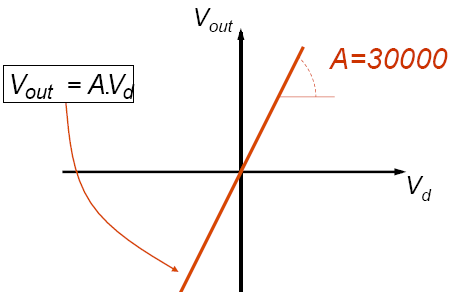
\includegraphics[scale=0.25]{img/image42}
\captionof{figure}{Caractéristique AOP}
\end{wrapfigure}
\subsubsection{Caractéristiques de transfert}

Un AOP possède plusieurs caractéristiques, mais nous nous intéressons ici à la \textit{caractéristique de transfert} c'est à dire le rapport entre la tension d'entrée $V_d$ et la tension de sortir $V_{out}$. Cette relation est déjà connue comme la loi fondamentale de l'AOP, loi qui se traduit par une droite de pente $A$.

\subsubsection{Caractéristique : zone linéaire}
\begin{wrapfigure}[7]{l}{3cm}
	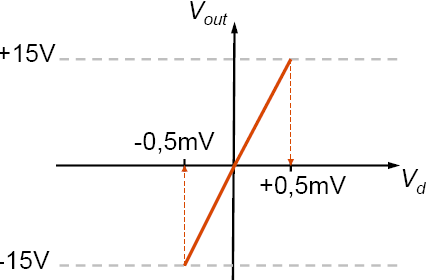
\includegraphics[scale=0.25]{img/image43}
	\captionof{figure}{Zone linéaire}
\end{wrapfigure}
Il ne faut pas oublier de tenir compte d'un phénomène supplémentaire, à savoir :
\begin{equation}
	-V_{al} \leq V_{out} \leq +V_{al}
\end{equation}
Ces limites se traduisent pas des horizontales dans le plan de la caractéristique. Seule la zone entre ces horizontales est accessible : il s'agit de la \textbf{zone linéaire}.\\
Les limites de cette zone sont simples à calculer, il s'agit des points de sortie pour lesquels $V_{d} = +V_{al}/A$ et $-V_{al}/A$. La grande valeur de $A$ a pour conséquence que la zone linéaire est très étroite sur l'axe horizontal.

\subsubsection{Caractéristique : saturation}
\begin{wrapfigure}[8]{r}{3cm}
	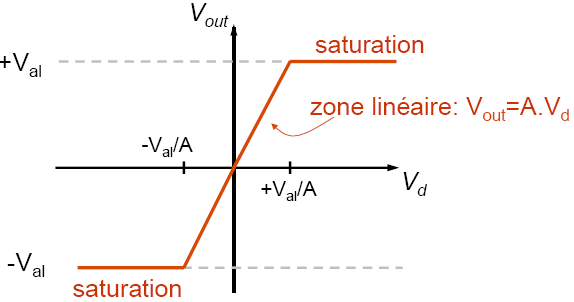
\includegraphics[scale=0.25]{img/image44}
	\captionof{figure}{Saturation}
\end{wrapfigure}
Si la tension d'entrée est au-dessus de $+V_{al}/A$, la tension de sortie est \textit{limitée} à la valeur $+V_{al}$ : l'AOP ne peut aller plus haut que sa propre tension d'alimentation positive (et pareil pour la tension négative). Dans ces deux cas, lorsque l'on sort de la zone linéaire on dit que l'AOP \textbf{sature}.\\
\textbf{Attention !} Dans les zones de saturations, la loi fondamentale n'est plus vérifiée : il n'y a plus d'amplification.




\subsubsection{Principe du zéro virtuel}
Il s'agit d'une propriété générale de tous les AOP, propriété directement liée à la caractéristique de ce dernier. Cette propriété fondamentale permet de faire gagner beaucoup de temps et s'énonce :\\

\prop{\textsc{Principe du zéro virtuel :} Tant qu'un amplificateur opérationnel \textbf{ne sature pas}, sa tension différentielle d'entrée est virtuellement nulle.}\ \\

Il est important de ne considérer cette théorique seulement si l'AOP est en zone linéaire (\textbf{erreur classique!}). Une tension différentielle virtuellement nulle signifie que $V_d$ est tellement faible que l'on peut la négliger devant les autres tensions (souvent, $V_d \ll 1\ mV$). Négliger $V_d$ signifie l'approximation :
\begin{equation}
	V_d = 0\ V
\end{equation}
C'est cette approximation que l'on appelle \textit{zéro virtuel}.\footnote{Zéro car $V_d$ est nulle, virtuel pour rappeler l'approximation.}


\subsubsection{Principe du zéro virtuel : remarques}
Quelques remarques sont à prendre en compte :
\begin{enumerate}
	\item Compte tenu de la définition de $V_d$, le zéro virtuel revient encore à faire l'approximation :
	      \begin{equation}
	      	V^+ = V^-
	      \end{equation}
	\item La grande valeur de $A$ justifie ce principe. En effet, dans la zone linéaire $V_d$ est négligeable ce qui est évident au moment de tracer la caractéristique de transfert.
	\item Le principe ne garantit \textbf{pas} que l'AOP est dans la zone linéaire.
	\item Si l'on suit le principe, la tension d'entrée est nulle, or c'est elle que l'on veut amplifier... Problem ? No ! Le zéro virtuel fait \textbf{simultanément} deux approximations :
	      \begin{enumerate}
	      	\item $V_d = 0\ V$
	      	\item $A = \infty$
	      \end{enumerate}
	      La loi fondamentale devient une "forme indéterminée" et la valeur n'est pas forcément nulle; pas de contradictions.
	\item Si l'on fait une des deux approximation du point précédent sans faire l'autre, on est foutu.
\end{enumerate}

\begin{wrapfigure}[9]{r}{3cm}
	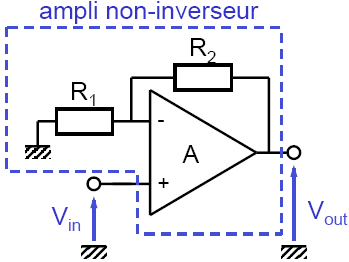
\includegraphics[scale=0.45]{img/image45}
	\captionof{figure}{Schéma non-inverseur}
\end{wrapfigure}
\section{Deux montages amplificateurs}
\subsection{Ampli non-inverseur}
Un montage amplificateur non-inverseur est un ampli-op auquel on a ajouté deux résistances $R_1$ et $R_2$ dans le but de "contrôler" le gain. 

\subsubsection{Montage >< composant}
Il est fondamental de faire la différence entre "deux" niveau du schéma : l'AOP qui est le composant et le montage construit sur base de cet AOP. C'est l'ensemble complet que l'on appelle \textit{amplificateur non-inverseur}. Son signal d'entrée est $V_{in}$, son signal de sortie $V_{out}$. Ces deux tensions sont référencées à la masse, elle sont donc \textbf{non-}différentielles.\\

Sur la figure du schéma non-inverseur, la résistance $R_2$ placée entre la sortie de l'AOP et son entrée inverseuse : elle est en \textbf{rétroaction}. 


\subsubsection{Calcul du gain $A_{\text{non\_inv}}$}
Nous allons chercher à calculer le \textit{gain du montage} défini\footnote{$A_{\text{non\_inv}}$ est le gain "à vide", on suppose qu'aucune charge n'est connectée à la sortie du montage.} :
\begin{equation}
	A_{\text{non\_inv}} = \frac{V_{out}}{V_{in}}
\end{equation}
Pour calculer ce gain, il faut choisir le modèle d'AOP que l'on utilise dans les calculs. Faisons les hypothèses suivantes et démontrons une expression du gain :
\begin{itemize}
	\item Le gain $A$ est fini (élevé, mais pas infini).
	\item Son impédance d'entrée $Z_d$ est infinie.
	\item Son impédance de sortie est nulle.
\end{itemize}
\begin{proof}
	\ \\
	Considérons les deux relations fondamentales de départ, ré-écrite sous une seule identité :
	\begin{equation}
		\left\{\begin{array}{ll}
		V_{out} & = A.V_d\\
		V_d & = V^+ - V^-
		\end{array}\right.\ \ \ \ \ \ \ \Rightarrow\ \ \ \ V_{out} = A.(V^+ - V^-)
	\end{equation}
	Essayons d'éliminer $V^+$ et $V^-$ au profit de $V_{in}$ et $V_{out}$ qui sont les variables à garder en finale. Comme $V_{in}$ est directement appliquée à l'entrée "+", on peut écrire :
	\begin{equation}
		V^+ = V_{in}
	\end{equation}
	On peut calculer $V^-$ par la méthodes des courants de branche, mais les propriétés de l'AOP permettent d'aller un peu plus vite. Posons qu'il existe un courant $I$ traversant $R_2$. Lorsque ce courant quitte $R_2$, il ne peut rentrer dans l'AOP car l'impédance de celui-ci est infinie : $I$ doit donc passer en totalité dans la résistance $R_1$.
	
	\begin{center}
		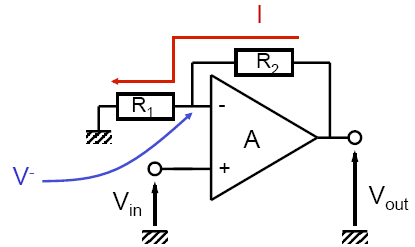
\includegraphics[scale=0.45]{img/image46}
		\captionof{figure}{Schéma pour le calcul de $V^-$}
	\end{center}
	
	En appliquant la loi d'Ohm sur chacune des résistances, on peut éliminer $I$ pour obtenir notre troisième équation : 
	\begin{equation}
		\left\{\begin{array}{ll}
		V^- & = R_1I\\
		V_{out} - V^- & = R_2I\\
		\rightarrow V_{out} & = (R_1+R_2)I
		\end{array}\right.\ \ \ \ \ \ \ \Rightarrow\ \ \ \ V^- = \dfrac{R_1}{R_1+R_2}V_{out}
	\end{equation}
	Notons que ce résultat aurait pu être immédiat par application du diviseur résistif, sous l'hypothèse que $Z_d = \infty$.\\ En combinant nos trois équations obtenues, on trouve l'équation
	\begin{equation}
		V_{out} = A\left(V_{in} - \dfrac{R_1}{R_1 + R_2}V_{out}\right)
	\end{equation}
	qu'il suffit de réarranger pour obtenir le gain recherché :
	\begin{equation}
		A_{\text{non\_inv}} = \frac{V_{out}}{V_{in}} = \frac{A(R_1+R_2)}{AR_1+R_1+R_2}
	\end{equation}
	La valeur élevée de $A$ permet de négliger $R_1$ et $R_2$ par rapport à $AR_1$. On trouve finalement le gain de notre AOP :\\
	
	\prop{$A_{\text{non\_inv}} \approx 1 + \frac{R_2}{R_1}$}
\end{proof}

\subsubsection{Amplificateur non-inverseur : remarques}
Si ce montage est dit "non-inverseur", c'est parce que son gain est positif. On remarque également que le gain de l'AOP ($A$) n'est pas dans l'expression de $A_{\text{non\_inv}} \rightarrow$ le gain du montage ne dépend pas du gain de l'AOP mais uniquement des valeurs des deux résistances. Les deux sous-sections précédentes sont consacrées à deux de ses propriétés.

\subsubsection{Montage non-inverseur à gain variable}
Régler le gain peut être fondamental, comme par exemple pour régler le volume de votre amplificateur audio. Pour se faire, il suffit de remplacer une des deux résistances (le plus souvent $R_2$, car étant au numérateur elle donne une variation linéaire du gain) par un \textit{potentiomètre}. Pour rappel :\\

\prop{Un potentiomètre est une résistance variable dont l'utilisateur règle la valeur via un curseur mécanique.}\ \\



%\subsubsection{Impédance d'entrée}

\subsection{Ampli inverseur}
\begin{wrapfigure}[7]{r}{3cm}
	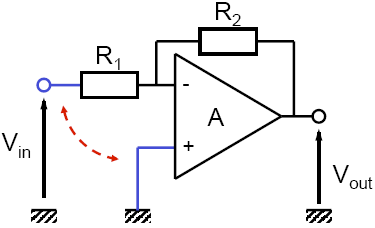
\includegraphics[scale=0.35]{img/image47}
	\captionof{figure}{Schéma inverseur}
\end{wrapfigure}
Ce montage à base d'un AOP est quasi-identique au non-inverseur à une exception près : le rôle de la masse et de l'entrée $V_{in}$ ont été permuté :
\begin{itemize}
	\item $V_{in}$ est maintenant connectée à $R_1$
	\item L'entrée "+" est maintenant mise à la masse
\end{itemize}
Notons cependant que $R_2$ est toujours montée en rétroaction (entre l'entrée et la sortie) et que $R_1$ et $R_2$ forment toujours un diviseur résistif (un peu particulier, car aucune des extrémités n'est à la masse).

\subsubsection{Calcul du gain $A_{inv}$}
En utilisant la méthode de calcul classique du point précédent (même hypothèses et démarches de calcul), on trouve que le gain à vide vaut :

\prop{\begin{equation}
	A_{inv} \approx -\frac{R_2}{R_1}
	\end{equation}}

\begin{proof}\ \\
	Afin de calculer la réponse en fréquence de ce circuit, il faut tout d'abord modéliser
	l'amplificateur opérationnel par un élément d'impédance d'entrée infinie, d'impédance
	de sortie nulle et de tension de sortie :
	    
	\begin{equation}
		V_{\text{out}}=A(V^+ - V^-)
	\end{equation}
	où A est le gain propre à l'amplificateur, très élevé, mais fini. Le gain à vide du montage
	étant:
	\begin{equation}
		G = \frac{V_{\text{out}}}{V_{\text{in}}}
	\end{equation}
	    
	Deux autres équations sont encore nécessaires pour arriver à  calculer le gain de notre
	amplificateur inverseur. Premièrement, nous savons que la borne positive est directement
	connectée à la masse. Deuxièmement, en utilisant la loi des mailles et en supposant qu'un
	même courant $I$ circule dans les résistances $R_1$ et $R_2$ (l'amplificateur possédant
	une impédance d'entrée infinie). Nous obtenons dès lors :
	
	\begin{equation}
		\left\{\begin{array}{l}
		V^+=0  \\
		V_{\text{in}}+R_1 I + R_2 I = V_{\text{out}}
		\end{array}\right.
	\end{equation}
	Sachant que $V^-=V_{\text{in}}+R_1 I$, nous obtenons l'équation :
	\begin{equation}
		V^-=V_{\text{in}}+R_1\frac{V_{\text{out}}-V_{\text{in}}}{R_1+R_2}
	\end{equation}
	
	Nous pouvons désormais exprimer $V_{\text{out}}$ en fonction de $V_{\text{in}}$ :
	\begin{equation}
		V_{\text{out}}=-A\left( \dfrac{V_{\text{in}}(R_1+R_2)+R_1 V_{\text{out}}-R_1 V_{\text{in}}}{R_1+R_2}\right) = -\dfrac{R_2 V_{\text{in}}+R_1 V_{\text{out}}}{R_1+R_2}
	\end{equation}
	Ou encore, après ré-arrangement :
	\begin{equation}
		(A R_1 + R_1 + R_2) V_{\text{out}} = -A R_2 V_{\text{in}}
	\end{equation}
	En supposant que $A R_1$ est beaucoup plus grand que $R_1 + R_2$, nous pouvons exprimer le 
	gain de notre amplificateur inverseur :
	\begin{equation}
		G =-\frac{A R_2}{A R_1 + R_1 + R_2} \approx -\frac{R_2}{R_1}
		\label{eq:gain}
	\end{equation}
\end{proof}

\subsubsection{Amplificateur inverseur : remarques}
Si ce montage est dit "inverseur" c'est parce que son gain est négatif. Comme pour le non-inverseur, le gain $A$ à également disparu de l'expression de $A_{inv}$. Comme avant, le gain peut être rendu variable à l'aide d'un potentiomètre si ce n'est qu'ici le gain minimal est nul !

\newpage
\subsubsection{Impédance d'entrée : calcul}
\begin{wrapfigure}[8]{l}{3.5cm}
	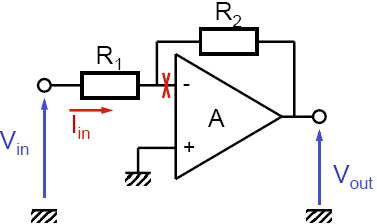
\includegraphics[scale=0.35]{img/image48}
	\captionof{figure}{Calcul de $Z$}
\end{wrapfigure}
Calculons l'impédance d'entrée du montage inverseur. 
\begin{equation}
	Z_{in} = \frac{V_{in}}{Z_{in}}\left|_{I_{out} = 0}\right.
\end{equation}
Le courant $I_{in}$ circulant n'est autre que celui circulant dans $R_1$, mais également celui circulant dans $R_2$ (l'impédance de l'AOP étant infinie). On peut donc écrire que ce courant vaut (loi d'Ohm sur l'ensemble des deux résistances) :
\begin{equation}
	I_{in} = \frac{V_{in} - V_{out}}{R_1+R_2}
\end{equation}
Par définition de l'AOP inverseur, $V_{out}$ vaut :
\begin{equation}
	V_{out} = A_{inv}.V_{in} = -\frac{R_2}{R_1}V_{in}
\end{equation}
En combinant les deux équations fraichement trouvées, on trouvé la valeur de $I_{in}$
\begin{equation}
	I_{in} = \frac{V_{in} + \frac{R_2}{R_1}V_{in}}{R_1+R_2} = \frac{V_{in}}{R_1}
\end{equation}
L'impédance d'entrée vaut dès lors :
\begin{equation}
	Z_{in} = R_1
\end{equation}
Il ne faut surtout pas conclure que l'impédance d'entrée du \textbf{montage} c'est "l'impédance qui se trouve à l'entrée du montage", résultat totalement faux dans le cas général ! Il faut dire que $Z_{in}$ à la même valeur que $R_1$ (sans l'être).\\

Cette impédance d'entrée est donc relativement faible (on pouvait s'attendre à ce qu'elle soit très élevée au vu de l'analyse du non-inverseur) doit être vue comme un inconvénient du montage inverseur.

\subsubsection{Méthode de calcul classique}
La méthode de résolution que nous avons utilisé tout au long du chapitre permet de résoudre tout circuit AOP avec rétroaction. Elle permet de calculer le gain à vide mais aussi de calculer l'impédance d'entrée sous hypothèses que l'impédance d'entrée d'un AOP soit aussi hight que Buzz.

\subsection{Calcul rapide par le principe du zéro virtuel}
Le principe du zéro virtuel énoncé précédemment permet d'effectuer un calcul beaucoup plus rapide qu'avec la méthode classique\footnote{Cela implique qu'on suppose $A = \infty$ dès le départ.}.

\newpage
\subsubsection{Calcul du gain de l'AOP non-inverseur}
\begin{wrapfigure}[8]{r}{3.5cm}
	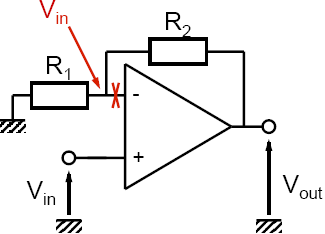
\includegraphics[scale=0.35]{img/image49}
	\captionof{figure}{AOP N-I}
\end{wrapfigure}
Commençons par poser nos différentes hypothèses sur l'AOP : impédance différentielle $Z_d$ infinie, impédance de sortie null et l'on a un zéro virtuel (gain de l'AOP infini et $V_d = 0$).\\
La "loi" n'est \textbf{plus} à utiliser ici ! De plus utiliser $A$ peut poser problème (comme supposé infini). A la place, ayant un zéro virtuel, on peut écrire $V^+ = V^- \rightarrow$ cette équation nous servira de "première équation". \\
Notre système d'équation est ainsi :
\begin{equation}
	\left\{\begin{array}{ll}
	V^+ &= V^-\\
	V^+ &= V_{in}\\
	V^- &= \frac{R_1}{R_1+R_2}V_{out}
	\end{array}\right.
\end{equation}
En vertu de la première équation, on peut immédiatement égaler les deux équations de droite et trouver directement le gain du montage
\begin{equation}
	A_{non_inv} = \frac{V_{out}}{V_{in}} = 1+\frac{R_2}{R_1}
\end{equation}
Ce qui est bien le même que celui obtenu avec la méthode classique.\\

C'est bien beau, mais on peut encore faire mieux en raisonnant "directement sur le schéma" tout en limitant les développement mathématiques :
\begin{enumerate}
	\item Dans l'hypothèse du zéro virtuel, $V^- = V^+$
	\item Or $V^+$ vaut $V_{in}$, ceux-ci étant en connexion directe
	\item Donc, $V^-$ vaut $V_{in}$
	\item Par ailleurs, $R_1$ et $R_2$ forment un diviseur résistif (car aucun courant ne passe dans l'AOP ($Z_d = \infty$)
	\item Pour ce diviseur résistif, on peut donc écrire
	      \begin{equation}
	      	V_{in} = \frac{R_1}{R_1+R_2}V_{out}
	      \end{equation}
	      Dont on déduit directement le gain
	      \begin{equation}
	      	A_{non_inv} = \frac{V_{out}}{V_{in}} = 1+\frac{R_2}{R_1}
	      \end{equation}
\end{enumerate}

En terme de rapidité, on ne peut faire mieux ! Mais : il faut bien maîtriser les concepts de la théorie et les appliquer au bon moment! 

\subsubsection{Calcul du gain de l'AOP inverseur}
\begin{wrapfigure}[8]{r}{3.5cm}
	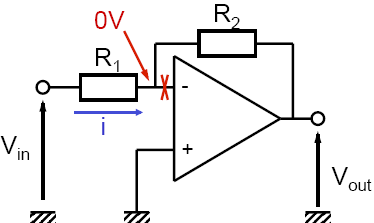
\includegraphics[scale=0.35]{img/image50}
	\captionof{figure}{AOP I.}
\end{wrapfigure}
Travaillons directement sur le schéma :
\begin{enumerate}
	\item Dans l'hypothèse du zéro virtuel, $V^- = V^+$
	\item Or $V^+$ vaut $0V$ : connexion directe à la masse
	\item Donc $V^-$ vaut 0 $V$ (on parle de "masse virtuelle")
	\item Par ailleurs, $R_1$ et $R_2$ forment un diviseur résistif (car aucun courant ne passe dans l'AOP ($Z_d = \infty$) (non "classique" car on a 0V au milieu des deux résistances)(j'aime les parenthèses)
	\item Le courant dans $R_1$ est facile à trouver :
	      \begin{equation}
	      	I = V_{in}/R_1
	      \end{equation}
	      En effet, comme l'extrémité droite de $R_1$ est (virtuellement à à la masse, la ddp sur $R_1$ vaut bien $V_{in}-0V = V_{in}$.
	\item Comme ce même courant passe dans $R_2$, on peut écrire : $0V~-~V_{out}~=~ R_2I$. On trouve finalement
	      \begin{equation}
	      	V_{out} = -R_2I = -R_2\left(\frac{V_{in}}{R_1}\right)
	      \end{equation}
	      ou encore
	      \begin{equation}
	      	A_{inv} = \frac{V_{out}}{V_{in}} = - \frac{R_2}{R_1}
	      \end{equation}
\end{enumerate}


	\subsection{Analyse de la rétroaction}
	Les deux montages vu précédemment comportent tous deux une résistance $R_2$ 
	en rétroaction. Clarifier le fonctionnement de cette rétroaction peut 
	répondre à un certains nombres de questions : pourquoi amplifier $V_d$ et 
	pas $V_{in}$, que justifie l'hypothèse du zéro virtuel ?
	
		\subsubsection{Analyse de la rétroaction : principe}
		Au cours de notre raisonnement, nous adopterons deux règles :
		\begin{enumerate}
			\item Raisonner strictement en termes de "cause" et d'"effet"
			\item L'AOP régit avec un certain délai : raisonnons plus vite que 
			lui ; supposons que la tension de sortie de l'AOP ne peut subir de 
			discontinuité (échelon)
		\end{enumerate}
		Ce dernier poins signifie que la tension de sortie ne peut pas varier 
		instantanément.	Nous allons considérer le cas d'un AOP non-inverseur de 
		gain $\approx 100$, $R_1 = 1k\Omega, R_2 = 99k\Omega$ et le gain de 
		l'AOP : $30000$.
		
		
		\subsubsection{Echelon sur $V_{in}$}
		Appliquons un échelon de $10mV$ sur $V_{in}$. Dans l'immédiat, $V^-$ 
		reste à 0V (pas de raison pour que ça change). Par contre, $V_d$ est 
		instantanément modifié : $V_d = V^+-V^- = 10mV$. Notre \textit{première 
		conséquence} de l'augmentation de $V_{in}$ est celle de $V_d$.
		
		\subsubsection{Conséquence de l'échelon $V_{out}$}
		\begin{wrapfigure}[8]{l}{8cm}
		\vspace{-8mm}
		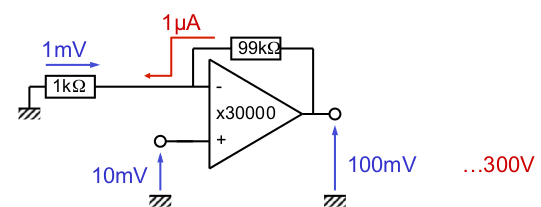
\includegraphics[scale=0.4]{ch4/image1}
		\captionof{figure}{ }
		\end{wrapfigure}
		A priori, la tension de sortie devrait être de 300V, mais ce n'est pas
		réaliste car l'AOP exploserait mais il se passe quelque chose : on 
		considère que la sortie croit linéairement et on analyse le moment ou 
		$V_{out} = 100mV$.\\
		Comme $V_{out}\neq 0$, du courant circule entre les deux $R$. Si rien 
		ne rentre dans l'AOP (impédance d'entrée infinie) ce courant vaut 
		\begin{equation}
		I = \dfrac{100mV}{100k\Omega} = 1\mu A
		\end{equation}
		Ce courant crée sur $R_1$ une chute de tension de $1k\Omega*1\mu A = 
		1mV$. Or, cette chute n'est autre que $V^-$ qui vaut donc $1mV$.
		
		\subsubsection{Conséquence de l'échelon : remarques}
		$R_1$ et $R_2$ forment un diviseur résistif\footnote{l'hypothèse $Z_{in} = 
		\infty$ est indispensable pour avoir le même courant dans les deux 
		résistances.} ; ici, $V^-$ sera toujours 100 fois plus faible que 
		$V_{out}$.
		
		\subsubsection{Conséquence de l'échelon : analyse}
		Au final, $V^-$ a bien été modifié mais pas directement par $V_{in}$. 
		Or, si $V^-$ change, $V_d$ également et vaut $9mV$. La rétroaction 
		réagit en sens inverse : augmenter $V^+$ fait diminuer $V_d$ via une 
		augmentation de $V^-$. Un "cycle" s'est formé.
		
		\subsubsection{Phase de "convergence"}
		On répète le cycle plusieurs fois, mais quand s’arrêter ? On 
		s'arrête quand la tension de sortie de l'AOP vaut exactement 
		3000*$V_d$. C'est cohérent, car à force de "boucler" il apparaissait 
		clairement que $V_d \rightarrow 0$.
		
		\subsubsection{Situation finale : remarques}
		Au final, $V_{out}$ vaut bien 100 fois $V_{in}$. De plus, la sortie 
		de l'AOP n'a jamais saturé : ceci justifie le zéro virtuel. Théorie 
		encore appuyée car $V_d$ est bien extrêmement faible, $V^+\approx 
		V^-$. On se doute bien qu'en réalité, ce phénomène est très rapide. 
		Nos équations ne nous informent donc que sur l'état d'équilibre 
		final du système.
		
		\subsubsection{Conclusion}
		\begin{itemize}
		\item[$\bullet$] \textit{A quoi sert la rétroaction par $R_2$ ?}\\
		Assure que $V^-$ "poursuit $V^+$, assurant le zéro virtuel. 
		Qualitativement, c'est elle qui fixe le gain.
		\item[$\bullet$] \textit{A quoi sert l'AOP ?}		\\
		Il assure que $V_{out}$ augmente quand $V_d$ augmente.
		\end{itemize}


		\subsubsection{Notion de "rétroaction négative"}
		La rétroaction ci-dessus est dite "négative" car elle contrecarre 
		toute variation de $V_d$. Si les variations de $V_d$ étaient 
		amplifiées, on parlerait de \textit{rétroaction positive}.



	\subsection{Compléments sur la rétroaction}
	Les deux montages vu comportent tous deux une rétroaction, on va ici 
	tenter de généraliser cette notion.
		
		\subsubsection{Montage $A$}
		\begin{wrapfigure}[5]{r}{8cm}
		\vspace{-8mm}
		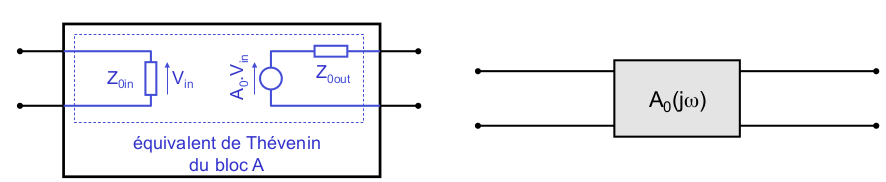
\includegraphics[scale=0.3]{ch4/image2}
		\captionof{figure}{ }
		\end{wrapfigure}
		Considérons un montage $A$ de gain $A_0$ que l'on définit par 
		son équivalent de Thévenin : impédance d'entrée $Z_{0in}$, de 
		sortie $Z_{0out}$ et de gain $A_0$. Pour simplifier, on va 
		considérer que $A_0 \in \mathbb{R}$ et plus généralement, le 
		gain est une \textit{fonction de transfert} $A_0(j\omega)$.
		
		\newpage
		\subsection{Gain en boucle ouverte}
		\begin{wrapfigure}[3]{r}{5cm}
		\vspace{-7mm}
		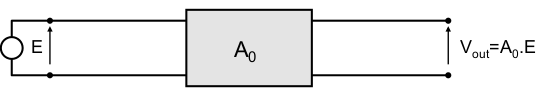
\includegraphics[scale=0.3]{ch4/image3}
		\captionof{figure}{ }
		\end{wrapfigure}
		Appliquer un signal $E$ au bloc $A$ multiplie le signal par 
		$A_0$. Rebaptisons $A_0$ le gain en boucle ouverte.
		
		\subsubsection{La rétroaction : définition}
		\begin{wrapfigure}[4]{l}{5cm}
		\vspace{-7mm}
		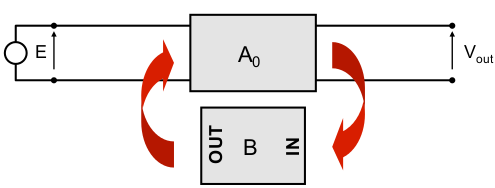
\includegraphics[scale=0.3]{ch4/image4}
		\captionof{figure}{ }
		\end{wrapfigure}
		Appliquer une rétroaction sur $A$, c'est prendre sa grandeur 
		de sortie pour la réinjecter, après passage dans un bloc $B$, 
		à l'entrée du bloc $A$ (où $B$ est défini par $B(j\omega)$). 
		Appliquer une rétroaction, c'est former une boucle fermée.\\
		
		On a ainsi créé un nouveau montage aux propriétés différentes 
		du bloc $A$ seul : le gain de montage est le \textit{gain en 
		boucle fermée}, $A_R$, différent du \textit{gain en boucle 
		ouverte} en l'absence de rétroaction.
		
		\subsubsection{Montage avec rétroaction}
		\begin{wrapfigure}[4]{r}{5cm}
		\vspace{-7mm}
		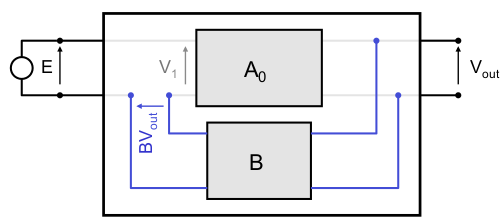
\includegraphics[scale=0.3]{ch4/image5}
		\captionof{figure}{ }
		\end{wrapfigure}
		On va maintenant calculer les propriétés de ce nouveau 
		montage, avec Thévenin. A droite du schéma ci-contre, on 
		prélève la tension de sortie du bloc $A_0$ ($V_{out}$) et ) 
		droite, on réinjecte la tension de sortie du bloc $B$ (
		$B.V_{out}$) \textbf{en série} avec la tension de source $E$.
		
		\subsubsection{Rétroaction de tension : calcul du gain $A_R$}
		Le gain en boucle fermée $A_R$ est défini comme
		\begin{equation}
		A_R = \left.\dfrac{V_{out}}{E}\right|_{I_{out}=0} 
		\end{equation}
		On a d'une part $V_{out} = A_0*V_1$ et d'autre part $V_1 = 
		E+B.V_{out}$. En combinant ces deux réactions : 
		\begin{equation}
		\left. \begin{array}{ll}
		V_{out} &= A_0.V_1\\
		V_1 &= E+B.V_{out}
		\end{array}\right\}\Rightarrow V_{out} = A_0(E+B.V_{out})\quad 
		\Longrightarrow A_R = \dfrac{V_{out}}{E}=\dfrac{A_0}{1-A_0B}
		\end{equation}
		
		\subsubsection{Rétroaction de tension: impédances}
		Comment les impédances d'entrées et de sorties sont-elles 
		influencées par l'ajout d'une rétroaction? On peut montrer que 
		\begin{equation}
		\begin{array}{ll}
		Z_{R_{in}} &= (1-A_0B)Z_{0_{in}}\\
		Z_{R_{out}} &= \dfrac{Z_{0_{out}}}{1-A_0.B}
		\end{array}
		\end{equation}
		On remarque que le facteur $1-A_0.B$ apparaît un peu partout. 
		L'effet d'une rétroaction sur à travers un bloc $B$ consiste à :
		\begin{itemize}
		\item[$\bullet$] Diviser le gain par $1-A_0B$
		\item[$\bullet$] Diviser l'impédance de sortie par $1-A_0B$
		\item[$\bullet$] Multiplier l'impédance d'entrée par $1-A_0B$
		\end{itemize}
		
		
		\subsubsection{Rétroaction négative}
		Quand $B<0$, la rétroaction est dite \textit{négative} (C.S.)
		\footnote{Si $A_0>0$}. Les propriétés d'une telle rétroaction 
		sont de diminuer le gain, mais augmenter les impédances pour 
		une adaptation en tension.
	
	
		\subsubsection{Rétroaction négative: ampli non-inverseur}
		Ce montage est un cas particulier de rétroaction négative. 
		Pour un tel montage, nous avons 
		\begin{equation}
		V_{out} = A\left(V_{in}-\dfrac{R_1}{R_1+R_2}V_{out}\right)
		\end{equation}
		Connaissant l'équation générale de la rétroaction de 
		tension $A_0(E+B.V_{out})$, on peut identifier :
		\begin{equation}
		\left\{\begin{array}{ll}
		A_0 &= A\\
		B &= -\dfrac{R_1}{R_1+R_2}
		\end{array}\right.
		\end{equation}
		Et donc
		\begin{equation}
		A_R = \dfrac{A_0}{1-A_0B} = \dfrac{A(R_1+R_2)}{AR_1+R_1+R_2}
		\end{equation}
		
		\subsubsection{Forte rétroaction négative}
		Lorsque $1\ll A_0.|B|$, la rétroaction est dite fortement 
		négative : $1-A_0B = A_0|B|$. Les propriétés sont identiques 
		au cas de la rétroaction négative.\\
		Le montage non-inverseur correspond à une forte rétroaction 
		négative : $B <0$ et $1\ll A_0.|B|$ car $A$ très élevé. En 
		appliquant directement la formule du gain en boucle fermée, 
		on retrouve bien le gain de l'ampli non-inverseur.
		
		\subsubsection{Rétroaction positive: définition intuitive}
		\begin{itemize}
		\item[$\bullet$] \textit{Rétroaction négative}
			\begin{itemize}
			\item Diminution du gain, la rétroaction s'oppose aux 
			perturbation du signal d'entrée, système stable
			\end{itemize}
		\item[$\bullet$] \textit{Rétroaction positive}
			\begin{itemize}
			\item Augmentation du gain, la rétroaction amplifie les 
			perturbations du signal d'entrée, système instable
			\end{itemize}
		\end{itemize}

\section{Montages à OPA}
La grande diversité des fonctions proposés par les montages à OPA 
réside dans la rétroaction. De tels montages agissent sur des 
grandeurs analogiques, même si ils peuvent véhiculé une information 
logique ou numérique. Regroupons ici, les diverses fonctions remplies 
par la bête en trois catégories.
	
	\newpage
	\subsection{Amplificateurs}
	\begin{wrapfigure}[9]{l}{7.1cm}
	\vspace{-0.5cm}
	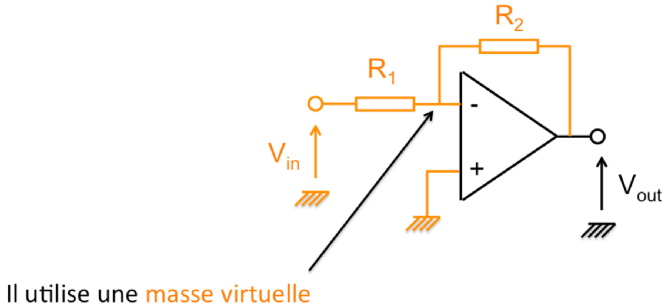
\includegraphics[scale=0.3]{ch4/image6}
	\captionof{figure}{AOP en montage inverseur}
	\end{wrapfigure}
	L'amplificateur non-inverseur amplifie un signal, dont le gain est
	\begin{equation}
	A = 1 + \dfrac{R_2}{R_1}
	\end{equation}
	si l'on considère le même schéma que précédemment. Le montage 
	inverseur fait de même, mais avec un gain en rétroaction 
	de :
	\begin{equation}
	A = -\dfrac{R_2}{R_1}
	\end{equation}
	L'intérêt du montage inverseur réside dans la présence d'une 
	masse virtuelle à l'entrée inverseuse impliquant que la ddp 
	sur $R_1$ soit $V_{in}$ et celle sur $R_2$ soit $-V_{out}$.\\
	
	\begin{wrapfigure}[9]{r}{2.4cm}
	\vspace{-1.2cm}
	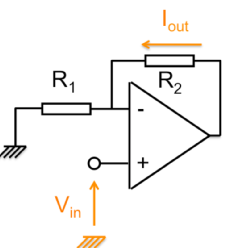
\includegraphics[scale=0.3]{ch4/image7}
	\captionof{figure}{Tension/courant}
	\end{wrapfigure}
	Ces deux montages permettent aussi la conversion tension $\rightarrow$ courant. 
	En effet, le courant dans $R_2 \propto V_1/R_1$ : il est 
	indépendant de $R_2$. Si l'on considère que la grandeur de sortie 
	$I_{out}$, le courant traversant $R_2$, en considérant $R_2$ comme 
	charge on a bien un convertisseur tension/courant.\\
	
	Le convertisseur tension $\rightarrow$ courant assure aussi la conversion inverse. 
	En injectant du courant dans $R_2$ ($Z_{entree}=\infty$), la tension 
	de sortie, $V_{out}$, doit forcément être $\propto$ au courant $I_{in}$.
	
	\begin{center}
		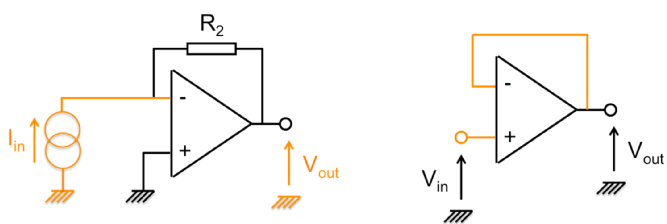
\includegraphics[scale=0.43]{ch4/image8}
	\captionof{figure}{Convertisseur courant/tension à gauche, suiveur à 
	droite}
	\end{center}
	Il existe aussi le "suiveur", un montage particulier non-inverseur 
	d'un gain $A=1$. Son avantage est de ne pas modifier le signal et son 
	utilité est de pouvoir résoudre des soucis d'adaptation d'impédance en 
	tension.
	
	
	\subsection{Circuits opérationnels}
	\begin{wrapfigure}[9]{r}{4.4cm}
	\vspace{-1.2cm}
	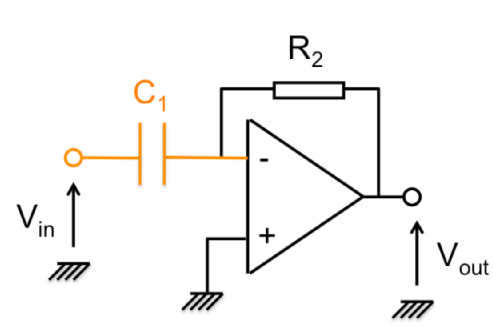
\includegraphics[scale=0.27]{ch4/image9}
	\captionof{figure}{Dérivation}
	\end{wrapfigure}
	On utilise ici l'OPA pour faire des opérations mathématique, d'où son 
	joli nom \textit{opérationnel}. Commençons par l'intégration : il faut 
	tout d'abord remplacer l'impédance de rétroaction $Z_2$ par une 
	capacité qui réalise cette fonction "intégration" : la tension à ses 
	bornes est directement lié à la tension d'entrée du montage $V_{in}$. 
	On peut ainsi convertir une onde carrée en onde triangulaire ! 
	\begin{equation}
	V_{C_2} = \dfrac{Q}{C}\qquad \text{ avec }\qquad Q = \int I\ dt = \int 
	\dfrac{R_1}{V_{in}}\ dt
	\end{equation}		
	\newpage
	Pour la 
	dérivation, il faut permuter les impédances. Cela se "voit" directement 
	en calculant la tension de sortie
	\begin{equation}
	V_{out} = -R_2C_1\left(\dfrac{\text{d}V_{in}}{dt}\right)
	\end{equation}
		\begin{wrapfigure}[7]{r}{4cm}
	\vspace{-0.5cm}
	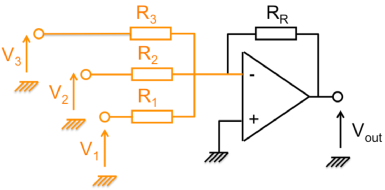
\includegraphics[scale=0.35]{ch4/image10}
	\captionof{figure}{Sommateur}
	\end{wrapfigure}
	On peut également créer un sommateur de $N$ tensions avec un circuit 
	inverseur. Par la loi des nœuds, le courant dans l'impédance $R_R$ est 
	la somme des courants parcourant les différentes impédances $R_i$. Cette 
	somme peut être pondérée en jouant sur la valeurs de $R_i$. On peut 
	également trouver la tension moyenne ou une amplification simultanée en 
	réglant $R_R$.\\
	
	\begin{wrapfigure}[9]{l}{5cm}
	\vspace{-0.5cm}
	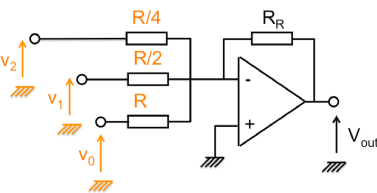
\includegraphics[scale=0.35]{ch4/image11}
	\captionof{figure}{Analogique/Numérique}
	\end{wrapfigure}
	Une autre fonction fondamentale est le convertisseur numérique/
	analogique	en utilisant le principe du sommateur : on divise chacune des 
	résistances d'entrée par un multiple de 2. Chacune des tension d'entrées 
	est binaire : 0 ou 1 V. Ci-contre, un cas à trois bits (3 tensions) formant un 
	mot binaire. La tension de sortie ne peut prendre que huit valeurs différentes ($2^3$).
	\begin{equation}
	V = \dots + 2^2 v_2 + 2^1v_1 + 2^0 v_0
	\end{equation}
	
	\subsection{Comparateurs}
	\begin{wrapfigure}[9]{r}{3.5cm}
	\vspace{-0.5cm}
	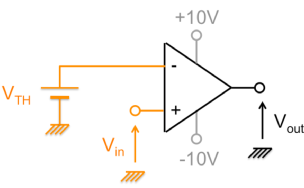
\includegraphics[scale=0.35]{ch4/image12}
	\captionof{figure}{Comparateur}
	\end{wrapfigure}
	Le but est de comparer une tension d'entrée $V_{in}$ par rapport à
	un seuil $V_{Th}$ et envoyer une information binaire (+10V ou -10V) 
	si oui ou non, cette tension est supérieur au seuil. \\
	L'idée est d'exploiter le fait que l'AOP sature dès qu'il sort de sa zone 
	linéaire, zone très étroite $(<1\ mV)$. Si la tension s'écarte du seuil 
	l'AOP sort de sa zone linéaire et sature à la tension d'alimentation 
	correspondante.\\
	\danger Ce montage ne comporte pas de rétroaction et ne respecte pas le 
	zéro virtuel ! On peut le voit comme un convertisseur A/N à un bit de 
	sortie.\\

	\begin{wrapfigure}[9]{l}{4cm}
	\vspace{-0.98cm}
	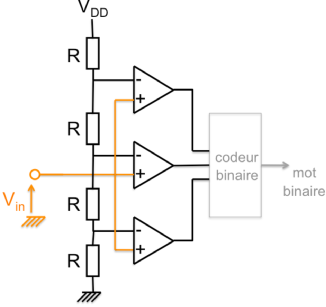
\includegraphics[scale=0.35]{ch4/image13}
	\captionof{figure}{Flash}
	\end{wrapfigure}	
	Ce précédent principe peut être utilisé pour créer un convertisseur A/N 
	de type FLASH : on mets plusieurs comparateurs à seuils régulièrement 
	espacés, mis en place via un dispositif résistif (pour avoir des seuils 
	différents). On peut alors "catégoriser" le signal d'entrée en fonction 
	de quels AOP ont saturés ou non. L'analyse de la sortie permet de déduire 
	l'intervalle de la tension d'entrée et convertir cette information en 
	binaire.\\

	\begin{wrapfigure}[6]{r}{4cm}
	\vspace{-0.98cm}
	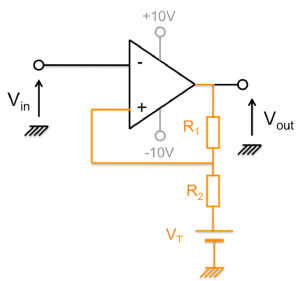
\includegraphics[scale=0.35]{ch4/image14}
	\captionof{figure}{Schmitt}
	\end{wrapfigure}		
	Si l'entrée est bruitée, notre comparateur pourrait indiquer une fausse 
	information et perturber l'appareil en aval. Créer une hystérèse\footnote{
	Cycle dans la caractéristique du composant.} permet d'éviter ces 
	oscillations : c'est le \textit{trigger de Schmitt}. L'idée est de créer 
	deux seuils différent, selon que $V_{in}$ croit ou décroît. On introduit 
	une hystérèse en ajoutant une instabilité via une rétroaction 
	\textbf{positive}. La borne $V_+$ est celle avec laquelle va être comparé 
	$V_{in}$. La rétroaction positive modifie $V_+$ dès que le seuil est 
	franchi dans un sens pour qu'une légère variation ne la fasse pas 
	"rebasculer" dans l'autre sens.\\
	
	Bien sûr, il existe d'autres montages : ampli d'isolation, filtres actifs, 
	isolateurs,\dots Ce qu'il faut retenir est que tout est dans la 
	rétroaction !
	
	
\section{L'AOP $\mathbb{R}$}
	\subsection{Imperfections statiques}
	Les variations de fréquences peuvent un peu tout foutre en l'air. Le terme 
	\textit{statique} désigne les basses fréquences, dont le continu. Nous allons 
	ici étudier les différentes imperfections.
	
		\subsubsection{L'offset}
		\begin{wrapfigure}[9]{r}{4cm}
		\vspace{-0.98cm}
		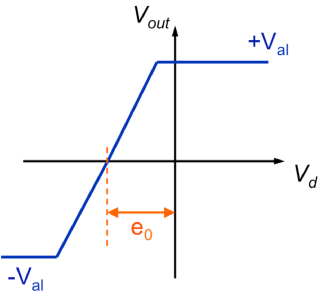
\includegraphics[scale=0.35]{ch4/image15}
		\captionof{figure}{Offset}
		\end{wrapfigure}	
		Il s'agit d'un décalage en tension de la caractéristique de transfert : 
		une tension continue vient s'ajouter au signal. Pour l'AOP, cela se 
		manifeste par un décalage horizontal de la caractéristique de 
		transfert, qui ne passe plus par l'origine : la sortie n'est plus 
		nulle si la tension appliquée l'est. Comme cette tension "s'ajoute", 
		la caractéristique se retrouve bien translatée vers la gauche. Parfois, 
		celui-ci est tellement grand que même une tension différentielle nulle 
		fait saturer notre bête !
		Pour le compenser, on peut ajouter à $V_d$ une tension d'entrée 
		correctrice (qu'il faut souvent réajuster, l'offset étant fonction de $T$).
		
		\subsubsection{Courants d'entrée}
		Les entrées de l'AOP bouffent ou vomissent un léger courant, pas forcément 
		identique\footnote{On les note souvent $i^+$ et $i^-$ en fonction de 
		l'entrée}. Les datasheet reprennent souvent deux paramètres 
		\begin{enumerate}
		\item Courant de polarisation ($i_{biais}$) ; moyenne des courants d'entrée.
		\item Courant de décalage ($i_{offset}$) ; différence des courants d'entrée.
		\end{enumerate}
		\danger Cette notion n'a \textbf{rien} avoir avec celle d'impédance 
		d'entrée : ici cela traduit le fait que l'AOP, même sans tension, 
		consomme un courant supplémentaire. Ces tensions viennent de la consommation 
		de transistors bipolaires, constituants de l'AOP.
		
		\subsubsection{Modélisation des imperfections}
		\begin{wrapfigure}[10]{l}{4.5cm}
		\vspace{-0.5cm}
		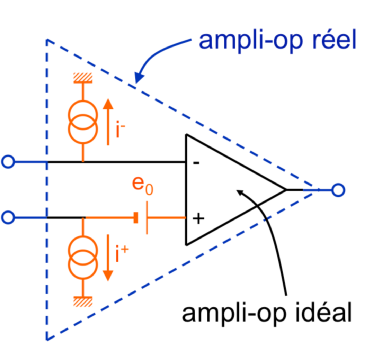
\includegraphics[scale=0.3]{ch4/image16}
		\captionof{figure}{AOP $\mathbb{R}$}
		\end{wrapfigure}	
		On considère le schéma d'un AOP idéal auquel on ajoute deux sources de 
		courant et une source de tension. Pour tenir compte de ces différents 
		effets, on applique la superposition : on annule les sources de tension 
		par un court circuit et les sources de courant par un circuit ouvert. Pour 
		appliquer ce principe, il faut faire l'hypothèse que l'AOP ne sature pas.\\
		
		On peut remarquer que lorsqu'on annule la tension d'entrée $V_{in}$, les 
		schémas inverseurs et non-inverseurs sont identiques.\\
		
		\newpage
			\begin{wrapfigure}[10]{l}{4.2cm}
		\vspace{-0.5cm}
		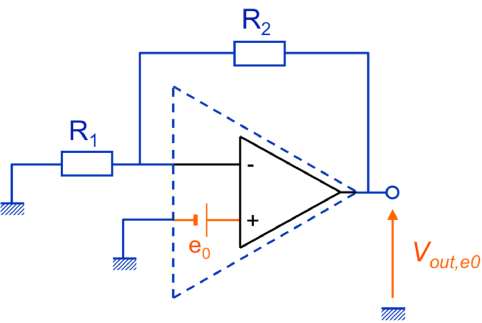
\includegraphics[scale=0.25]{ch4/image17}
		\captionof{figure}{ }
		\end{wrapfigure}
		Commençons par l'offset $e_0$ seul : on ouvre $i^-$ et $i^+$ et on court 
		circuite $V_{in}$. Après résolution, on trouve
		\begin{equation}
		V_{out,e_0} = A_{non-inv}*e_0
		\end{equation}
		Ce résultat est valable quelque soit le montage, même inverseur !\\
		
		Considérons maintenant les courants d'entrées. Le souci est que ces courants 
		circulent forcément, et ils le font dans les résistances ce qui crée une 
		perte de tension. L'effet est donc indirect : un offset. Ceci est illustré 
		ci-dessous (droite) par l'application d'une tension $V_{in}$ sur deux 
		résistances $R^\pm$.
		\begin{center}
		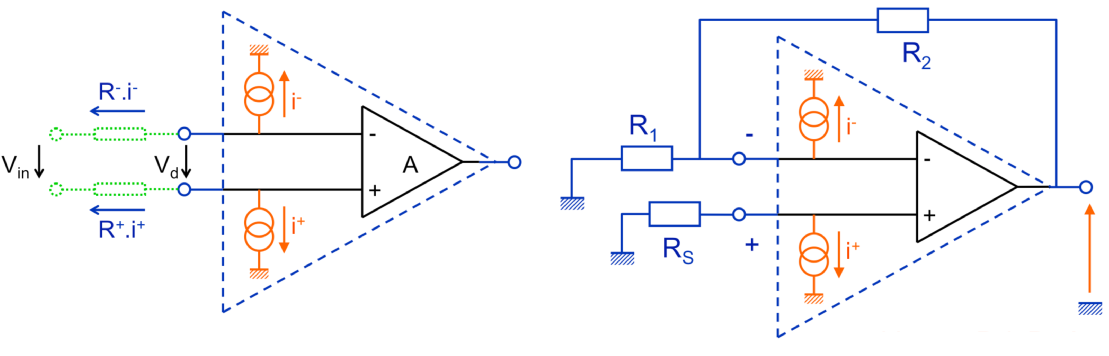
\includegraphics[scale=0.3]{ch4/image18}
		\captionof{figure}{ }
		\end{center}
		Forcément, nous avons
		\begin{equation}
		V_d = V_{in} + (R^-i^-)-(R^+i^+)
		\end{equation}				
		Si les deux résistances ou les courants ne sont pas identiques, la tension 
		est bien modifiée. Au sens de Thévenin, il s'agit de résistance d'entrée que 
		l'on nomme ici \textit{résistance de source}. Appliquons maintenant le 
		principe de superposition. Il faut commencer par voir quels sont les $R$ de 
		notre circuit :
		\begin{itemize}
		\item[$\bullet$] Entrée inverseuse : $i^-$ peut circuler via $R_1$ et/ou 
		$R_2$.
		\item[$\bullet$] Entrée non-inverseuse : on a pour l'instant juste la masse, 
		$V_{in}$ étant court-circuitée. Cependant, la source de tension n'est pas 
		parfaite et contient une résistance $R_S$ que l'on désigne \textit{résistance 
		de sortie}.
		\end{itemize}
		La résolution du circuit ci-dessus (droite) donne
		\begin{equation}
		V_{out_{i_{pol}}} = R_2i^- - R_SA_{non-inv}.i^+
		\end{equation}
		\danger Ici on ne peut pas considérer qu'aucun courant rentre dans l'AOP 
		$\mathbb{R}$ ! Mais cette hypothèse reste valable pour l'AOP idéal.\\
		
		On applique maintenant notre précieux théorème en sommant tout :
		\begin{equation}
		V_{out} = A_{non-inv}*V_{in} + A_{non-inv}*e_0 + R_2i^- - R_SA_{non-inv}.i^+
		\end{equation}
		Ce résultat n'est valable que si l'AOP ne sature \textbf{pas}. \danger Pour 
		un montage inverseur, seul le premier terme de gain change ! Les deux autres 
		sont identiques, les calculs étant valables pour les deux montages.\\
		
		\textbf{Question d'examen } :On donne un gain, courant, fréquence, \dots et on 
		donne qquelques AOP. Il faut choisir lequel est le plus adapté et pourquoi 
		(si on peut négliger quelque chose,\dots).
		
		\subsubsection{Imperfections statiques : plus loin !}
		On peut évidemment tenir compte d'autres imperfections comme par exemple 
		tenir compte de $Z_d$ et $Z_{out}$. On peut faire encore mieux en considérant 
		la tension en mode commun ; la moyenne des deux signaux. Même si on l'a 
		négligé, deux choses en dépendent 
		\begin{enumerate}
		\item La tension de sortie. L'idéal est d'avoir un \textit{taux de réjection 
		en mode commun"} (CMRR) le plus grand possible car cela signifie que cet 
		effet est petit.
		\item L'impédance d'entrée. Elle traduit le fait que l'AOP dépend aussi de 
		cette tension en mode commun qu'on lui applique.
		\end{enumerate}
		
	\subsection{Comportement fréquentiel}
		\subsubsection{Fonction de transfert d'un RC passe-bas}
		Il s'agit d'un circuit à un pôle étudier en long et en large au premier labo. 
		Sa fonction de transfert est la suivante
		\begin{equation}
		H(j\omega) = \dfrac{1}{1+j\omega RC}
		\end{equation}
		\begin{center}
		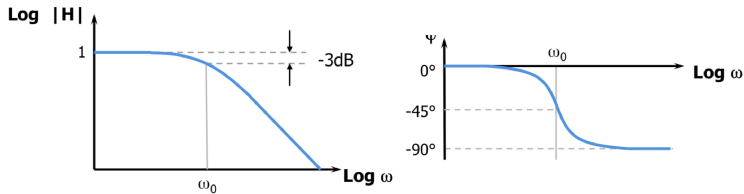
\includegraphics[scale=0.53]{ch4/image19}
		\captionof{figure}{Fonction de transfert d'un RC passe-bas}
		\end{center}
		En première approximation, l'AOP réel est un circuit à un pôle. Un AOP réel 
		comporte une impédance de sortie non-nulle et des capacités parasite. On 
		obtient alors un "montage" constitué d'un AOP idéal de gain $A_0$avec une 
		résistance et une capacité. La seule différence avec le circuit RC est le 
		gain $A_0$ : l'asymptote horizontale de $\log|H|$ vaudra dès lors $A_0$ et 
		non plus 1. L'AOP agit ainsi comme un filtre passe-bas : au delà d'une 
		certaine fréquence le gain diminue jusqu'à devenir nul.\\
		
		Quel est l'effet de la rétroaction sur la fonction de transfert? Soit un 
		montage non-inverseur. Pour calculer la fonction de transfert, on applique 
		les formules générales de la rétroaction :
		\begin{itemize}
		\item[$\bullet$] Bloc A : L'AOP à un pole. Fonction de transfert : $A(j\omega) 
		= A_0/(1+j\omega RC)$.
		\item[$\bullet$] Bloc B : La rétroaction. Fonction de transfert\footnote{Voir 
		plus haut, déjà étudié.} : $B(j\omega) = -R_1/(R_1+R_2)$.
		\end{itemize}
		Comme vu précédemment, la fonction de transfert du bloc $A$ avec une rétroaction 
		devient 
		\begin{equation}
		A_R(j\omega) = \dfrac{A(j\omega)}{1-A(j\omega).B(j\omega)}
		\end{equation}
		En première approximation, le gain est divisé par $1-A_0B$ et la pulsation de 
		coupure (et donc sa bande passante) est multipliée par ce même facteur. La fonction 
		de transfert voit donc 	son gain descendre et le graphique de la phase se voit translaté 
		vers la droite.
	
	
		\subsubsection{Produit "gain * bande passante"}
		On vient de le voir, une rétroaction augmente la bande passante. Comme un 
		même facteur intervient dans deux cas, on peut dire que le produit suivant, 
		le produit "gain * bande passante" est constant 
		\begin{equation}
		A_0'\omega_0' = A_0\omega_0
		\end{equation}
		Cela signifie qu'il n'est pas possible d'avoir à la fois un gain élevé et une 
		bande passante élevée mais aussi que ce produit, constant, est une caractéristique 
		intrinsèque de l'AOP.\\
		Pour l'info, on peut aussi modéliser l'AOP comme ayant trois pôles.
		
	\setcounter{subsection}{3}
	\subsection{Dimensionnement d'un montage à ampli-op}
	Il faut suivre ces quelques étapes ! Rajoutons qu'il est important de savoir 
	dimensionner un AOP en tant qu'ingénieur!
	\begin{enumerate}
	\item Établir le cahier des charges
	\item Calculer le nombre d'étages (via le produit gain * bande passante)
	\item Choisir le type d'étages (impédances et phase)
	\item Calculer les tensions de décalage en sortie (offset et courants d'entrée)
	\end{enumerate}
	
	
	
	
	
	
	
	
	
	
	
	
	
	
	
	
	
